\documentclass[11pt]{article}
\usepackage[utf8]{inputenc}
\usepackage{amsmath, amssymb, amsfonts}
\usepackage{geometry}
\usepackage{booktabs}
\usepackage{tikz}
\usetikzlibrary{quantikz}
\usepackage{braket}
\usepackage{float}

% --- Modern Bibliography Setup ---
% Use 'phys' style for physics formatting (AIP/APS)
\usepackage[style=phys, backend=biber, biblabel=brackets]{biblatex} 
\addbibresource{references.bib} 

% --- Clickable Links (Load this AFTER biblatex) ---
\usepackage[colorlinks=true, allcolors=blue]{hyperref}

\geometry{a4paper, margin=1in}

\setlength{\parindent}{0pt}

\title{Exact block encoded square matrices}
\author{Tree encoding square matrix data and calculating product and sum encodings}
\date{\today}

\begin{document}

\maketitle


%======================================================
%
%. Encoding a row using a tree data stucture
%
%======================================================

\section*{Encoding a row using a tree data structure}

The encoding af a row vector with complex entries is most easily explained with a low dimensional example. So let's do n = 3. \\

Consider a 3 dimensional complex row vector $r = (\alpha1,\alpha2,\alpha3)$. 
The row vector will be encoded as a 2 qubit state, so we make the replacement  $r = (\alpha1,\alpha2,\alpha3,0)$ \\

From the vector $r$ the following tree is constructed
\begin{center}
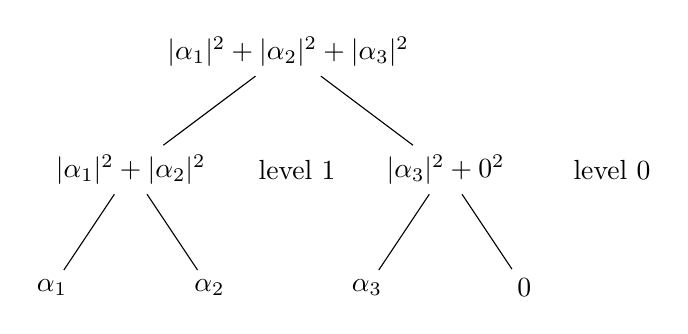
\begin{tikzpicture}[level distance=1.5cm,
  level 1/.style={sibling distance=4cm},
  level 2/.style={sibling distance=2cm}]
  \node {$|\alpha_1|^2 + |\alpha_2|^2 + |\alpha_3|^2$}
    child {node {$|\alpha_1|^2 + |\alpha_2|^2$}
      child {node {$\alpha_1$}}
      child {node {$\alpha_2$}}
      node[right=1.5cm] {level 1}
    }
    child {node {$|\alpha_3|^2 + 0^2$}
      child {node {$\alpha_3$}}
      child {node {$0$}}
      node[right=1.5cm] {level 0}
    };
\end{tikzpicture}
\end{center}

For each pair of leaves and internal nodes on each a unitary is constructed
\[
R(\alpha, \beta) = \frac{1}{N_{\alpha\beta}} \begin{bmatrix} \alpha & -\beta^* \\ \beta & \alpha \end{bmatrix}
\]
properly normalised by the Frobenius norm of the matrix $N_{\alpha\beta}$. \\

In the $n=3$ case we define the unitaries
\begin{align*}
R &= R(\sqrt{|\alpha_1|^2 + |\alpha_2|^2}, \sqrt{|\alpha_3|^2}) \\
R_0 &= C^0 R(\alpha_1, \alpha_2) = (X \otimes I)(CR(\alpha_1, \alpha_2))(X \otimes I) \\
R_1 &= C^1 R(\alpha_3, 0) = CR(\alpha_3, 0)
\end{align*}

The $C$'s are conditionals $C^1 = C$ on the first qubit being $|1\rangle$ and $C^0$ on the second qubit being $|0\rangle$. For deeper trees we need bit pattern conditionals e.g.
\[
C^{01} R = (X \otimes I \otimes I) C(CR) (X \otimes I \otimes I)
\]

In case thee $\alpha$'s are complex, the unitaries are composed of $Y$ and $Z$ rotations $Rz(\phi)Ry(\theta)Rz(\psi)$. But for real parameters, e.g. for internal nodes, they are pure $Y$-rotations. \\

The encoding is performed by the circuit
\begin{center}
\begin{quantikz}
\lstick{0} & \gate{R} & \octrl{1}   & \ctrl{1}   & \qw \\
\lstick{0} & \qw       & \gate{R_0} & \gate{R_1} & \qw
\end{quantikz}
\end{center}

In bra-ket notation we get the normalised state:

\begin{align*}
|00\rangle &\xrightarrow{R} \frac{1}{(|\alpha_1|^2 + |\alpha_2|^2 + |\alpha_3|^2)^{1/2}} \left( \sqrt{|\alpha_1|^2 + |\alpha_2|^2} |00\rangle + \sqrt{|\alpha_3|^2} |10\rangle \right) \\
&\xrightarrow{R_0} \frac{1}{(|\alpha_1|^2 + |\alpha_2|^2 + |\alpha_3|^2)^{1/2}} \left( \sqrt{|\alpha_1|^2 + |\alpha_2|^2} \frac{\alpha_1}{\sqrt{|\alpha_1|^2 + |\alpha_2|^2}} |00\rangle \right. \\
&\quad \left. + \sqrt{|\alpha_1|^2 + |\alpha_2|^2} \frac{\alpha_2}{\sqrt{|\alpha_1|^2 + |\alpha_2|^2}} |01\rangle \right) \\
&\xrightarrow{R_1} \frac{1}{(|\alpha_1|^2 + |\alpha_2|^2 + |\alpha_3|^2)^{1/2}} (\alpha_1 |00\rangle + \alpha_2 |01\rangle + \alpha_3 |10\rangle)
\end{align*}

Explain a few details about the algorithm ...


%======================================================
%
%. Encoding a matrix once the rows have been encoded
%
%======================================================

\section*{Encoding a matrix once the rows have been encoded}

The framework for these operations is detailed in the quantum recommendation systems paper by Kerenidis and Prakash \cite{KerenidisPrakash2017}.   ... mere detaljer her ...\\

For each row in a square the procedure in the preceeding paragraph results in an encoding of an i'th row state 
$$
|A_i \rangle = \frac{1}{\|A_i\|} \sum_j a_{ij} |j\rangle
$$

To encode the entire matrix once the rows have been encoded, two unitaries must be constructed $V$ and $U$ satisfying (the registers for $U$ have been swapped relative to references ...)
 \begin{align*}
    U : |0i \rangle & \to |i A_i \rangle = \frac{1}{\|A_i\|} \sum_j a_{ij} |ij\rangle \\
    V : |0j \rangle & \to |\tilde{A}_j j\rangle, \quad \tilde{A}_j = \|A\|_j / \|A\|
\end{align*}

The $V$ matrix effectively contains the normallization of each encoded row ...\\

That $U^\dagger V$ encodes the matrix, is proven by calculating the $ij$-th matrixelement of the projected matrix
 \begin{align*}
        \langle i| (\langle 0| \otimes I) U^\dagger V (|0\rangle \otimes I) |j\rangle &= \langle 0i| U^\dagger V |0j\rangle = \langle i A_i | \tilde{A}_j j \rangle \\
        &= \langle i | \tilde{A}_j \rangle \langle A_i | j \rangle = \frac{\|A_i\|}{\|A\|} a_{ij}^* / \|A_i\| = a_{ij}^* \frac{1}{\|A\|}
    \end{align*}

So actually to prepare a complex matrix, we begin by encoding the complex conjugate of the rows. \\


%------------------------------------------------------------------------
%      Explicit construction of U
%------------------------------------------------------------------------
\subsection*{Explicit construction of $U$}

We continue the $n=3$ case, starting with the matrix representation. \\

Given the three $4 \times 4$ row encoding matrices $R_1, R_2, R_3$, we define the $16 \times 16$ block diagonal matrix $\tilde{U}$ as:
\[
\tilde{U} = \begin{bmatrix}
R_1 & 0 & 0 & 0 \\
0 & R_2 & 0 & 0 \\
0 & 0 & R_3 & 0 \\
0 & 0 & 0 & I_2
\end{bmatrix}
\]
The $4\times4$ identity matrix $I_2$ (the 2 qubit identity) comes from the $0$-padding prior to preparing the rows. \\

We also need the permutation matrix, $P_{swap}$, corresponding to a register swap (see Dirac notation below)
\[
P_{swap} = \begin{bmatrix}
I_2 & 0 & 0 & 0 \\
0 & 0 & I_2 & 0 \\
0 & I_2 & 0 & 0 \\
0 & 0 & 0 & I_2
\end{bmatrix}
\]

To obtain the matrix $U$, we multiply $\tilde{U}$ on the right by $P_{swap}$
\[ U = \tilde{U} \cdot P_{swap} \]

In bra-ket notation the $16 \times 16$ space as two 2-qubit registers $\mathcal{H}_1 \otimes \mathcal{H}_2$.
The block diagonal matrix $\tilde{U}$ is:
\[ \tilde{U} = \sum_{i=0}^3 \ket{i}\bra{i} \otimes R_i \]

The permutation matrix $P_{swap}$ is the register swap operator:
\[ P_{swap} = \sum_{j=0}^3 \sum_{k=0}^3 \ket{j, k}\bra{k, j} \]

The resulting interleaved matrix $U = \tilde{U}P_{swap}$ acts on basis states as:
\[ U \ket{j, k} = \ket{k} \otimes (U_k \ket{j}) \]

If one wants to avoid direct sums, the matrix $U$ can be decomposed into a register swap followed by four doubly-controlled 2-qubit gates.

\begin{center}
\begin{quantikz}
\lstick{$q_3$} & \swap{2} & \octrl{2} & \octrl{2} & \ctrl{2}  & \ctrl{2}  & \qw \\
\lstick{$q_2$} & \swap{2} & \octrl{1} & \ctrl{1}  & \octrl{1} & \ctrl{1}  & \qw \\
\lstick{$q_1$} & \qw      & \gate[2]{R_1} & \gate[2]{R_2} & \gate[2]{R_3} & \gate[2]{I} & \qw \\
\lstick{$q_0$} & \qw      &           &           &           &           & \qw 
\end{quantikz}
\end{center}
(The last conditional obviously not necessary.)

%------------------------------------------------------------------------
%.       Explicit construction of V
%------------------------------------------------------------------------

\subsection*{Explicit construction of $V$}
To construct the $V$ matrix we start by row encoding the vector consisting of the Frobenius norm of each row
$$
r_{norm} = (\|A_1\|, \|A_2\|, \|A_3\|, 0)
$$
as a $4 x 4$ matrix $V_{norm}$ and then simply letting
$$
V = V_{norm} \otimes I_2 
$$


%======================================================
%
%             Product encoding
%
%======================================================

\section*{Product of Block Matrices}

And also by Gily\'{e}n, Su,  Low, and Wiebe,  \cite{GSLW2019}.  ... mere detaljer her ...\\

Diagramatically the product $U_{AB}$ of two $n$ qubit encodings $U_A$ and $U_B$ can be illustrated as

\begin{figure}[H]
\begin{center}
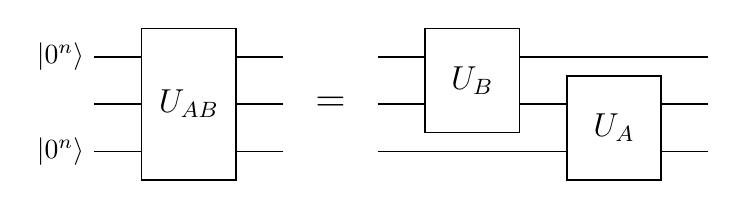
\begin{tikzpicture}[scale=1.2, line width=0.6pt]
% --- Left Side (U_AB) ---
\draw (0,2) -- (0.5,2); \node[left] at (0,2) {$\ket{0^n}$};
\draw (0,1.5) -- (0.5,1.5);
\draw (0,1) -- (0.5,1); \node[left] at (0,1) {$\ket{0^n}$};
\draw (0.5,0.7) rectangle (1.5,2.3);
\node at (1,1.5) {\large $U_{AB}$};
\draw (1.5,2) -- (2,2);
\draw (1.5,1.5) -- (2,1.5);
\draw (1.5,1) -- (2,1);
\node at (2.5,1.5) {\Large $=$};
% --- Right Side (U_B and U_A) ---
\draw (3,2) -- (3.5,2);
\draw (3,1.5) -- (3.5,1.5);
\draw (3,1) -- (5,1); 
\draw (3.5,1.2) rectangle (4.5,2.3);
\node at (4,1.75) {\large $U_{B}$};
\draw (4.5,2) -- (6.5,2);
\draw (4.5,1.5) -- (5,1.5);
\draw (5,0.7) rectangle (6,1.8);
\node at (5.5,1.25) {\large $U_{A}$};
\draw (6,1.5) -- (6.5,1.5);
\draw (6,1) -- (6.5,1);
\end{tikzpicture}
    \caption{This is a diagram drawn with TikZ.}
    \label{fig:tikz_example} % Must be after the caption
\end{center}
\end{figure}

But this way, the encoded matrix will not end up in the upper left corner ...\\

To make sure that the unitaries gets applied to the relevant qubits and to make sure that the encoded matrix ends up in the upper left corner, a couple of swap matrices needs to be introduced (alluded to in the papers ...)

\begin{equation*}
   U_{AB} = (I_n  \otimes  U_A \cdot P_{swap})   (U_B \otimes I_n) (I_n \otimes P_{swap})
\end{equation*}

In Dirac notation the proof is:
\begin{equation*}
\begin{aligned}
&\langle 0^n0^ni | (I_n \otimes P_{swap}) (I_n \otimes P_{swap} U_A P_{swap}) (U_B \otimes I_n) (I_n \otimes P_{swap}) | 0^n0^nj \rangle = \\
&\langle 0^ni0^n | (I_n \otimes P_{swap} U_A P_{swap}) (U_B \otimes I_n) | 0^nj0^n \rangle = \\
&\langle 0^n | \left( \langle 0^ni | U_A P_{swap} \right) \left( U_B | 0^nj \rangle \right) | 0^n \rangle = \\
&\langle 0^n | \otimes ( \langle 0^ni | U_A P_{swap} ) (|0^n\rangle \langle 0^n| \otimes I_n \otimes I_n) (I_n \otimes I_n \otimes |0^n\rangle \langle 0^n|) ( U_B | 0^nj \rangle \otimes |0^n\rangle ) = \\
&\langle 0^n | \otimes ( \langle 0^ni | U_A P_{swap} ) (|0^n\rangle \langle 0^n| \otimes I_n \otimes |0^n\rangle \langle 0^n|) ( U_B | 0^nj \rangle \otimes |0^n\rangle ) = \\
&\langle 0^n | \otimes ( \langle 0^ni | U_A P_{swap} ) \left( \sum_k |0^n\rangle \langle 0^n| \otimes |k\rangle \langle k| \otimes |0^n\rangle \langle 0^n| \right) ( U_B | 0^nj \rangle \otimes |0^n\rangle ) = \\
&\sum_k \langle 0^n0^ni | (I_n \otimes U_A P_{swap}) | 0^nk0^n \rangle \langle 0^nk0^n | (U_B \otimes I_n) | 0^nj0^n \rangle = \\
&\sum_k \underbrace{\langle 0^n0^ni | I_n \otimes U_A | 0^n0^nk \rangle}_{A_{ik}} \underbrace{\langle 0^nk0^n | (U_B \otimes I_n) | 0^nj0^n \rangle}_{B_{kj}} = (AB)_{ij}
\end{aligned}
\end{equation*}

To further appreciate the need for the register swaps, see the appendix, where the $2\times2$ case in matrix notation is shown in full detail.

%======================================================
%
%            Sum encoding
%
%======================================================

\section*{Sum of Block Matrices}

Flere detaljer her ... men det er ganske simpelt:
\begin{align*}
        W &= (X \otimes I) \cdot (C U_A) \cdot (X \otimes I) \cdot (C U_B) \\
             &= U_A  \oplus U_B \\
        U_{A+B} &= (P_L^{\dagger} \otimes I) \cdot W \cdot (P_R \otimes I)
\end{align*}



%======================================================
%
%               Example $2x2$ matrix calculation
%
%======================================================
\newpage

\section*{Appendix: Example $2 \times 2$ matrix calculation}
In this appendix we go through the matrix calculations for the simplest possible case of a product encoding: The case where we have (1,1,0)-encodings $U_A$ and $U_B$ of two $2 \times 2$ matrices $A$ and $B$. This serves to justify the need for the register swaps in the formula for the product encoding.\\

The projected matrix corresponding to the circuit in figure \ref{fig:tikz_example} is supposedly \footnote{Smith, J. (2023). Title of the Book. Publisher.}
$$
(\langle 0| \otimes I \otimes \langle 0|) (I \otimes U_A) (U_B \otimes I) (|0\rangle \otimes I \otimes |0\rangle)
$$
But this submatrix doesn't live in the upper left corner of it's unitary encoding.\\

We can fix that by applying register swaps $P_{swap}$ to get $\langle 0| \otimes I \otimes \langle 0| \to \langle 0|  \otimes \langle 0| \otimes I$ and similarly for the ket-state. \\

But we actually need more swaps for the matrices to affect the correct qubits. We will show exactly how in the following subsections.

\subsection*{Translating bra-kets to matrices}
The Kronecker product translates between Dirac notation and matrices : 
\begin{itemize}
    \item $\langle 0| = \begin{bmatrix} 1 & 0 \end{bmatrix}, \quad |0\rangle = \begin{bmatrix} 1 \\ 0 \end{bmatrix}$
   
    \item $\langle 0| \otimes I = \begin{bmatrix} I & 0 \end{bmatrix}$
    
      \item $I \otimes |0\rangle = \begin{bmatrix} 1 & 0 \\ 0 & 0 \\ 0 & 1 \\ 0 & 0 \end{bmatrix}$
\end{itemize}
All in all, we have
\begin{itemize}
    \item $\langle 0| \otimes I \otimes \langle 0| = \begin{bmatrix} 1 & 0 & 0 & 0 \\ 0 & 1 & 0 & 0 \end{bmatrix} \otimes 
     \begin{bmatrix} 1 & 0 \end{bmatrix} = 
    \left[ \begin{array}{cccc|cccc}
    1 & 0 & 0 & 0 & 0 & 0 & 0 & 0 \\
    0 & 0 & 1 & 0 & 0 & 0 & 0 & 0 
    \end{array} \right]$
    \item $|0\rangle \otimes I \otimes |0\rangle = 
    \begin{bmatrix} 
    1 & 0 \\ 0 & 0 \\ 0 & 1 \\ 0 & 0 \\ 0 & 0 \\ 0 & 0 \\ 0 & 0 \\ 0 & 0 
    \end{bmatrix}$
\end{itemize}
(We are using $=$ to suggest an identification)

\newpage
\subsection*{Finding the projected matrix}
Now we can calculate the projected matrix
\begin{align*}
&\langle 0| \otimes I \otimes \langle 0|) (I \otimes U_A) (U_B \otimes I) (|0\rangle \otimes I \otimes |0\rangle = \\ 
&\begin{bmatrix} 1 & 0 & 0 & 0 & 0 & 0 & 0 & 0 \\ 0 & 0 & 1 & 0 & 0 & 0 & 0 & 0 \end{bmatrix}
\begin{bmatrix} U_A & 0 \\ 0 & U_A \end{bmatrix}
\left[ \begin{array}{c|c} 
\begin{matrix} 
	u^B_{11} & 0 & u^B_{12} & 0 \\ 
	0 & u^B_{11} & 0 & u^B_{12} \\ 
	u^B_{21} & 0 & u^B_{22} & 0 \\ 
	0 & u^B_{21} & 0 & u^B_{22} 
\end{matrix}  & \dots \\ \hline \dots & \dots 
\end{array} \right]
\begin{bmatrix} 1 & 0 \\ 0 & 0 \\ 0 & 1 \\ 0 & 0 \\ 0 & 0 \\ 0 & 0 \\ 0 & 0 \\ 0 & 0 \end{bmatrix} = \\
&\begin{bmatrix} 
u^A_{11} & u^A_{12} & u^A_{13} & u^A_{14} & 0 & 0 & 0 & 0 \\
u^A_{31} & u^A_{32} & u^A_{33} & u^A_{34} & 0 & 0 & 0 & 0 
\end{bmatrix}
\begin{bmatrix}
u^B_{11} & u^B_{12} \\
0 & 0 \\ 
u^B_{21} & u^B_{22} \\
0 & 0 \\
\vdots & \vdots 
\end{bmatrix} = \\
&\begin{bmatrix}
u^A_{11}u^B_{11} + u^A_{13}u^B_{21} & u^A_{11}u^B_{12} + u^A_{13}u^B_{22} \\
u^A_{31}u^B_{11} + u^A_{33}u^B_{21} & u^A_{31}u^B_{12} + u^A_{33}u^B_{22}
\end{bmatrix} \\
\end{align*}
To make sure the resulting matrix is identical to the actual product $AB$ we must have
\begin{align*}
U_A = \begin{bmatrix} 
a_{11}& * &a_{12} & * \\
* & * & * & * \\
a_{21}& * & a_{22} & * \\
* & * & * & *
\end{bmatrix} & , 
U_B = \left[ \begin{array}{cc|c}
b_{11} & b_{12} & * \\
b_{21} & b_{22} & \\ \hline
* & & * 
\end{array} \right] 
\end{align*}
Notice $U_A$ is thus not a projected encoding of $A$. \\
We can fix this by replacing $U_A$ in equation... by
$$
\tilde{U}_A = P_{swap} \left[ \begin{array}{c|c} 
A & * \\ \hline 
* & * 
\end{array} \right] P_{swap}
$$
where here $P_{swap}$ is the $2$ register swap matrix
$$
\begin{bmatrix} 
1 & 0 & 0 & 0 \\ 
0 & 0 & 1 & 0 \\ 
0 & 1 & 0 & 0 \\ 
0 & 0 & 0 & 1 
\end{bmatrix}
$$


% --- Display the Modern Bibliography ---
\printbibliography

\end{document}
